\chapter{Технологический раздел}
В данном разеделе представлены выбор инструментов для реализации и оценки алгоритмов, а также листинги полученного кода.

\section{Требование к ПО}

К программе предъявляется ряд требований:

\begin{itemize}
	\item на вход подаётся объекта класса TriPolArray, состоящий из объектов (треугольных полигонов);
	\item на выходе — заполненные ZBuffer и FrameBuffer, содержащие соответственно глубины и цвета всех видимых точек на экране.
\end{itemize}

\section{Выбор инструментов}
По-скольку наиболее освоенным языком для разработчика является c++, для реализации алгоритмов был выбран именно он, т.к. таким образом работа будет проделана наиболее быстро и качественно.

Соответсвенно для компиляции кода будет использоваться компилятор G++.

Чтобы оценить время выполнения программы будет замерятся реальное время, т.к. таким образом можно будет сравнить реализации алгоритмов без и с использованием параллельных вычислений. Для замера реального времени работы программы используется функция clock() т.к. программа тестируется на компьютере с установленной ОС Windows. \cite{clock()}

Кроме этого, необходимо отключить оптимизации компилятора для более честного сравнения алгоритмов. В моём случае это делается с помощью ключа $-O0$ т.к. используется компилятор G++. \cite{optimization}

\section{Реализация алгоритмов}
На листингах \ref{ZBufferAlg::execute}-\ref{ZBufferAlg::executeWithTrheads} представлены реализации алгоритма ZBuffer без и с использованием параллельных вычислений.

\section{Тестирование}
Для проверки написанных алгоритмов были подготовлены следующие тесты:
\begin{itemize}
	\item проверка алгоритма ZBuffer
	\item проверка трёхмерного переноса
	\item проверка трёхмерного масштабирования
	\item проверка трёхмерного поворота
\end{itemize}

На рисунках \ref{start}-\ref{rotate} приведены результаты тестирования.

\begin{figure}[h]
	\center{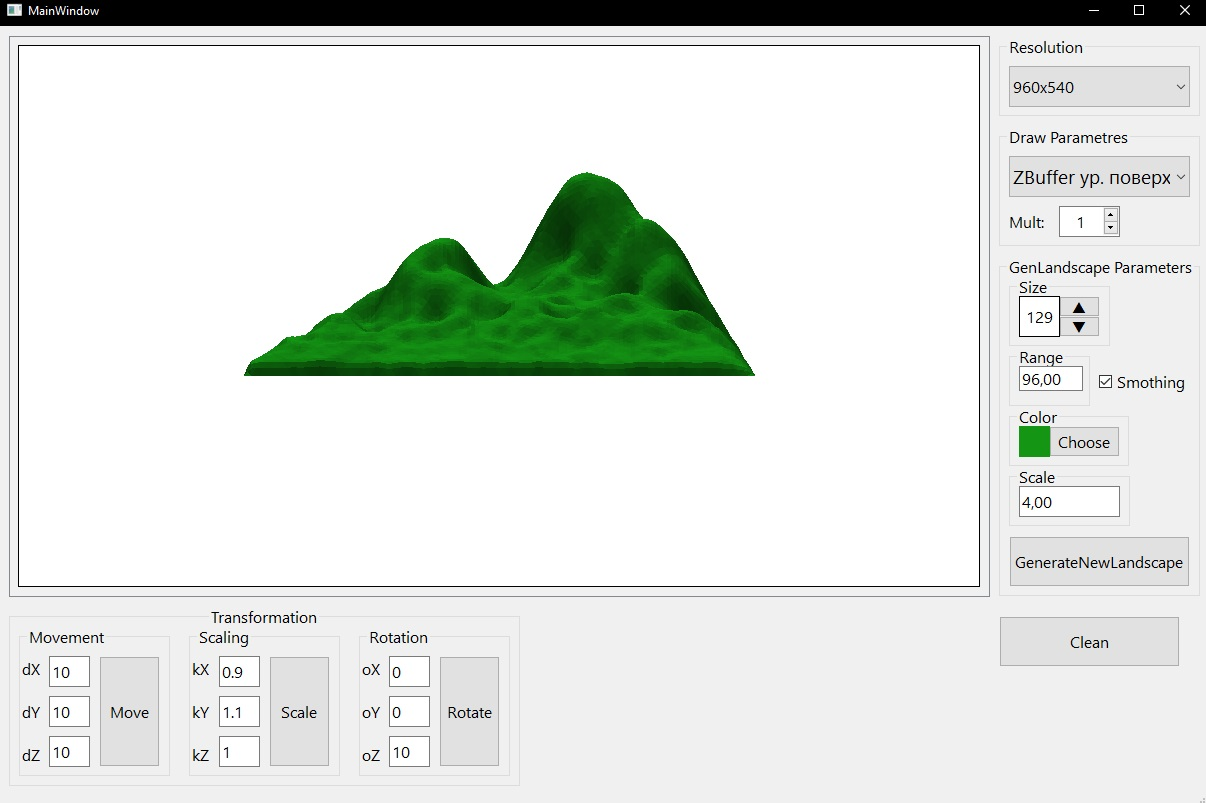
\includegraphics[width=1\linewidth]{inc/img/start}}
	\caption{Начальное положение ландшафта}
	\label{start}
\end{figure}

\begin{figure}
	\center{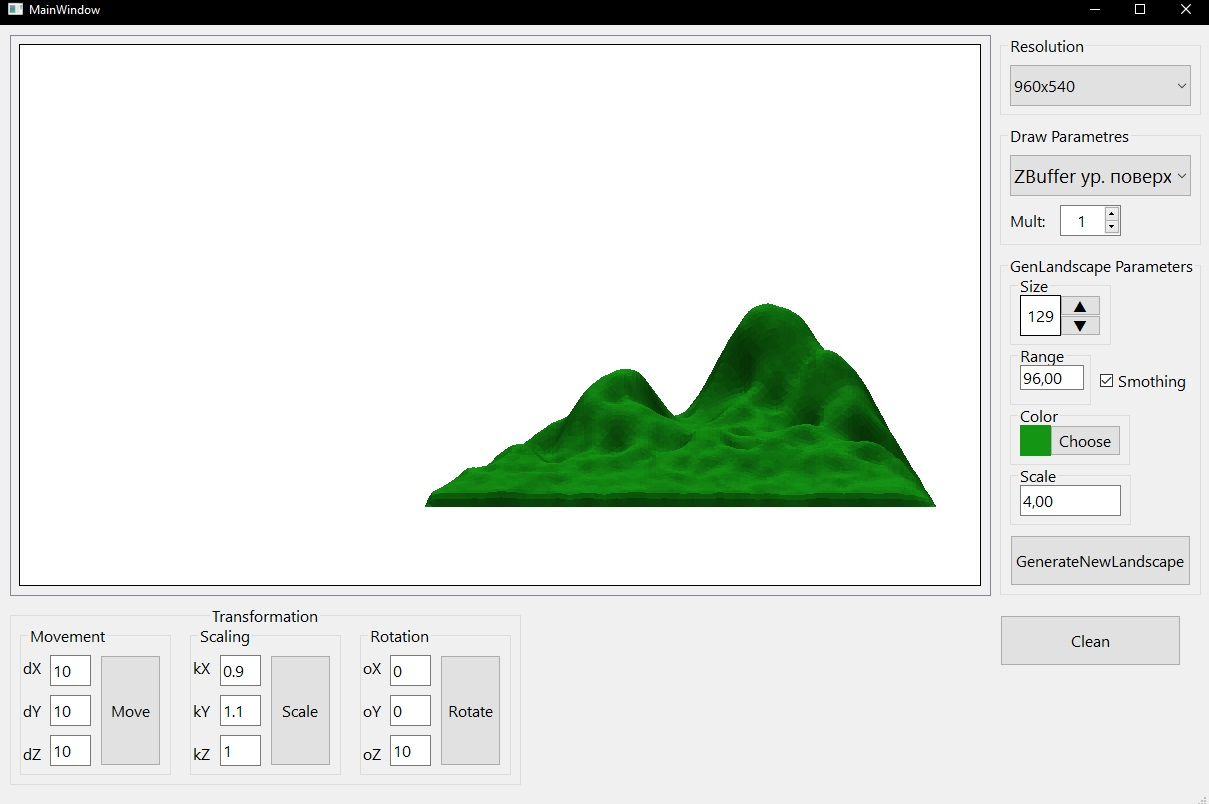
\includegraphics[width=1\linewidth]{inc/img/move}}
	\caption{Трёхмерный перенос ландшафта}
	\label{move}
\end{figure}

\begin{figure}
	\center{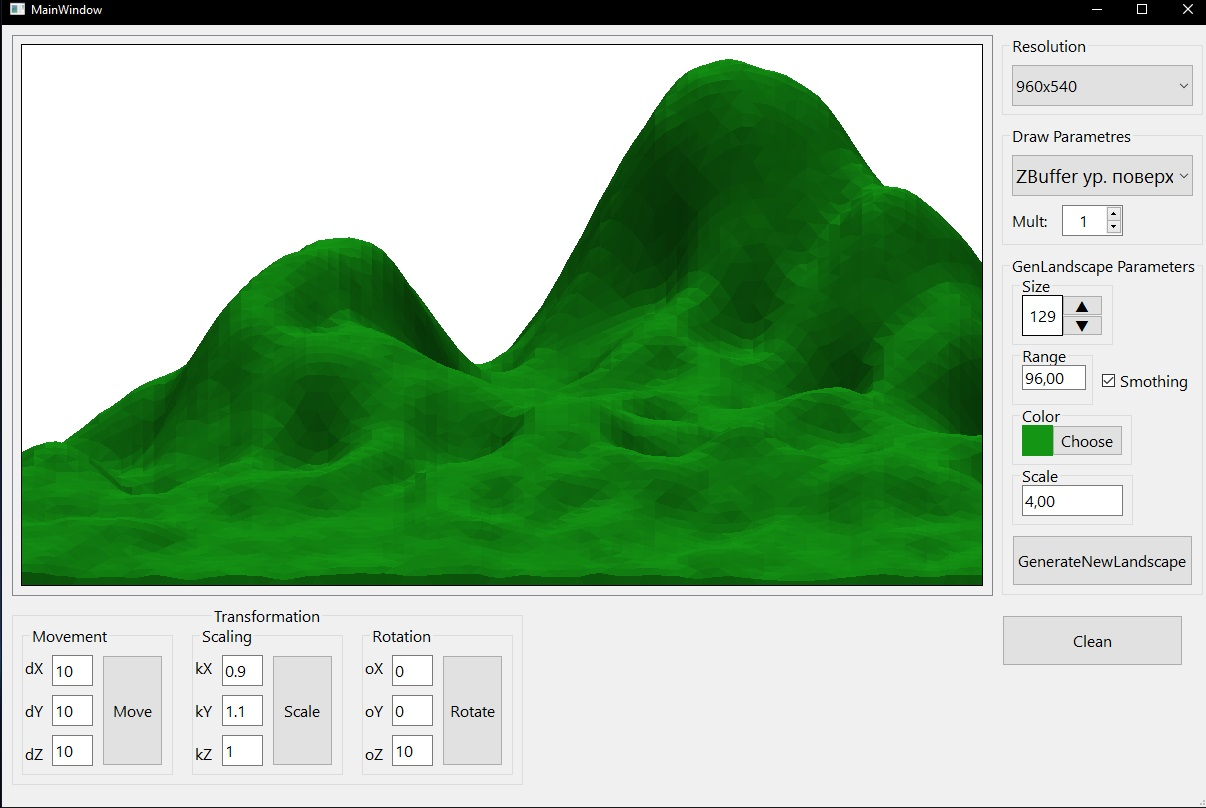
\includegraphics[width=1\linewidth]{inc/img/scale}}
	\caption{Трёхмерное масштабирование ландшафта}
	\label{scale}
\end{figure}

\begin{figure}
	\center{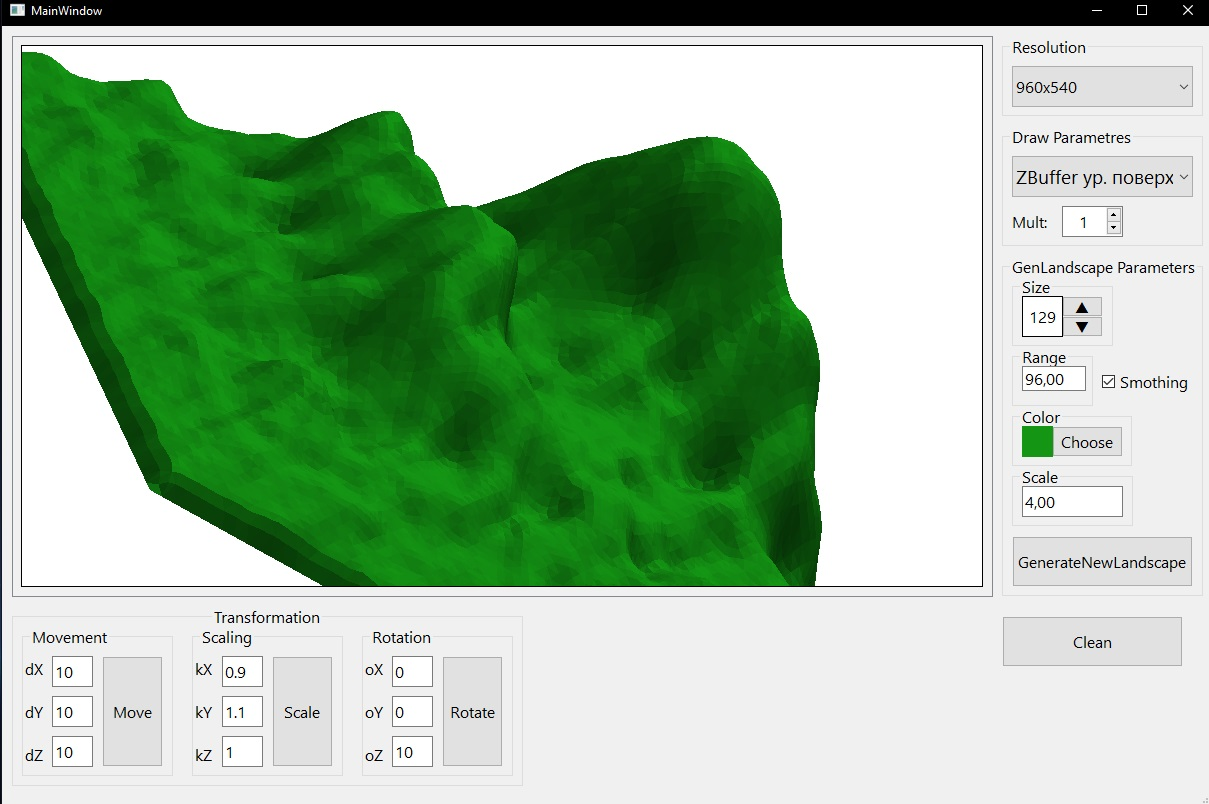
\includegraphics[width=1\linewidth]{inc/img/rotate}}
	\caption{Трёхмерный поворот ландшафта}
	\label{rotate}
\end{figure}

\newpage
Как видно по рисункам, все тесты пройдены.

\section{Вывод}
В данном разделе были выбраны инструменты для реализации выбранных алгоритмов, представлены листинги реализованных алгоритмов, а также проведено тестирование.